
%%%%%%%%%%%%%%%%%%%%%%%%%%%%%%%%%%%%%%%%%%%%%%%%%%%%%%%%%%%%%%%%%%%%%%%%%%%%%%%%%%%%%%%
%%%%%%%%%%%%%%%%%%%%%%%%%%%%%%%%%%%%%%%%%%%%%%%%%%%%%%%%%%%%%%%%%%%%%%%%%%%%%%%%%%%%%%%
% 
% This top part of the document is called the 'preamble'.  Modify it with caution!
%
% The real document starts below where it says 'The main document starts here'.

\documentclass[12pt]{article}

\usepackage{amssymb,amsmath,amsthm}
\usepackage[top=1in, bottom=1in, left=1.25in, right=1.25in]{geometry}
\usepackage{fancyhdr}
\usepackage{enumerate}
\usepackage{listings}
\usepackage{graphicx}
\usepackage{float}

\usepackage{mwe}
\usepackage{caption}
\usepackage{subcaption}
% Comment the following line to use TeX's default font of Computer Modern.
\usepackage{times,txfonts}



\makeatletter
\renewcommand*\env@matrix[1][*\c@MaxMatrixCols c]{%
  \hskip -\arraycolsep
  \let\@ifnextchar\new@ifnextchar
  \array{#1}}
\makeatother

\newtheoremstyle{homework}% name of the style to be used
  {18pt}% measure of space to leave above the theorem. E.g.: 3pt
  {12pt}% measure of space to leave below the theorem. E.g.: 3pt
  {}% name of font to use in the body of the theorem
  {}% measure of space to indent
  {\bfseries}% name of head font
  {:}% punctuation between head and body
  {2ex}% space after theorem head; " " = normal interword space
  {}% Manually specify head
\theoremstyle{homework} 

% Set up an Exercise environment and a Solution label.
\newtheorem*{exercisecore}{Exercise \@currentlabel}
\newenvironment{exercise}[1]
{\def\@currentlabel{#1}\exercisecore}
{\endexercisecore}

\newcommand{\localhead}[1]{\par\smallskip\noindent\textbf{#1}\nobreak\\}%
\newcommand\solution{\localhead{Solution:}}

%%%%%%%%%%%%%%%%%%%%%%%%%%%%%%%%%%%%%%%%%%%%%%%%%%%%%%%%%%%%%%%%%%%%%%%%
%
% Stuff for getting the name/document date/title across the header
\makeatletter
\RequirePackage{fancyhdr}
\pagestyle{fancy}
\fancyfoot[C]{\ifnum \value{page} > 1\relax\thepage\fi}
\fancyhead[L]{\ifx\@doclabel\@empty\else\@doclabel\fi}
\fancyhead[C]{\ifx\@docdate\@empty\else\@docdate\fi}
\fancyhead[R]{\ifx\@docauthor\@empty\else\@docauthor\fi}
\headheight 15pt

\def\doclabel#1{\gdef\@doclabel{#1}}
\doclabel{Use {\tt\textbackslash doclabel\{MY LABEL\}}.}
\def\docdate#1{\gdef\@docdate{#1}}
\docdate{Use {\tt\textbackslash docdate\{MY DATE\}}.}
\def\docauthor#1{\gdef\@docauthor{#1}}
\docauthor{Use {\tt\textbackslash docauthor\{MY NAME\}}.}
\makeatother

% Shortcuts for blackboard bold number sets (reals, integers, etc.)
\newcommand{\Reals}{\ensuremath{\mathbb R}}
\newcommand{\Nats}{\ensuremath{\mathbb N}}
\newcommand{\Ints}{\ensuremath{\mathbb Z}}
\newcommand{\Rats}{\ensuremath{\mathbb Q}}
\newcommand{\Cplx}{\ensuremath{\mathbb C}}
%% Some equivalents that some people may prefer.
\let\RR\Reals
\let\NN\Nats
\let\II\Ints
\let\CC\Cplx

%%%%%%%%%%%%%%%%%%%%%%%%%%%%%%%%%%%%%%%%%%%%%%%%%%%%%%%%%%%%%%%%%%%%%%%%%%%%%%%%%%%%%%%
%%%%%%%%%%%%%%%%%%%%%%%%%%%%%%%%%%%%%%%%%%%%%%%%%%%%%%%%%%%%%%%%%%%%%%%%%%%%%%%%%%%%%%%
% 
% The main document start here.

% The following commands set up the material that appears in the header.
\doclabel{STAT 401: Homework 8}
\docauthor{Stefano Fochesatto}
\docdate{\today}


%\begin{figure}[H]
%  \begin{center}
%  \caption{}
%  \includegraphics[\textwidth]{}
%  \end{center}
%\end{figure}

% \textbf{Code:}
% \begin{center}
% \lstinputlisting{}
% \end{center} 



\begin{document}

\begin{exercise}{1} Use the data lathe1 from problem 5.12 and do the following: 
  \begin{enumerate}
    \item[a.] As described in 5.12.2, fir the full second order model using log(Life) as the response and 
    speed and feed as the predictors. A full second-order model is one which includes both predictors, 
    second-order polynomial terms in both predicts, and the interaction term between the predicts. Report
    your fitted model. \\
    \solution The full second-order model es defined by, 
      \begin{equation*}
        Y = \beta_0 + \beta_1X_1 + \beta_2X_2 + \beta_3X^2_1 + \beta_4X^2_2 + \beta_5X^1X^2 + \epsilon
      \end{equation*}
      Fitting the model in r we get the following, \\
       \textbf{Code:}
       \begin{center}
       \lstinputlisting[basicstyle=\small]{r1.txt}
       \end{center} 
       \newpage


       \item[b.] Obtain the efedct plot for the interaciton between Speed and Feed in the full second-order model 
       you should see a series of quadratic curves which owing to the insignificance of the interaction term, essentially 
       match one another except separated by vertical shifts. \\
       \solution Using r to obtain the effect plot we get, 
        \begin{figure}[H]
          \begin{center}
          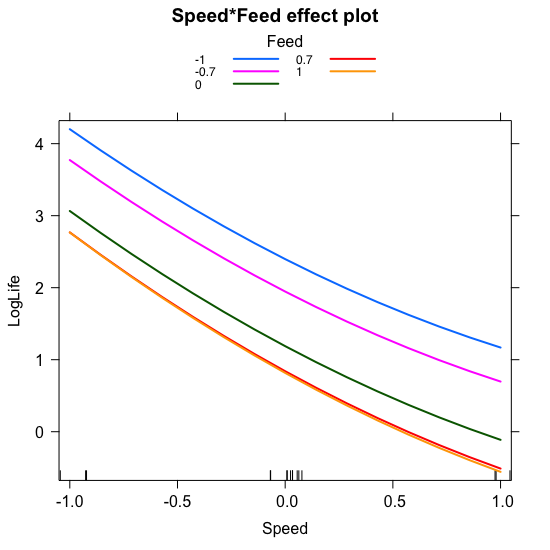
\includegraphics[width = .66\textwidth]{Rplot.png}
          \end{center}
        \end{figure}
        \textbf{Code:}
        \begin{center}
        \lstinputlisting[basicstyle=\small]{r2.txt}
        \end{center} 
        \newpage
        \newpage

        \item[c.] Test the interaction term in your model. You can use the coefficient's t-test 
        or perform a partial $F$ test using anova(). Does your result agree with what you're effect plot
        showed.\\
        \solution Performing partial $F$ test in r, using the anova() function we get the following, \\
        \textbf{Code:}
        \begin{center}
        \lstinputlisting[basicstyle=\small]{r3.txt}
        \end{center} 
        We can see that with a with a p-value of .4994, adding the interaction to the model does not provide a statistically
        significant improvement. This does match what our effect plot is telling us. The effect plot above described an inverse
        relationship between speed on log(life) and feed on log(life), these effect are likely cancelling each other out and we are 
        left with an insignificant parameter. 
        \newpage
        
        \item[d.] Remove the interaction term and refit the model. Test the quadratic terms in speed an feed to determine 
        if the first order model is adequate.  \\
        \solution Below is the partial $F$ tests for determining which second order terms should be included in the model. In general 
        all the squared terms contributed on the $\alpha = .05$ significance level to the model. The first test evaluates the second order
        speed term against the first order model. The second test evaluates the second order feed term against the first order model. The 
        next two test show us that of the two second order terms the feed term is most significant. Finally the last test compares the second order 
        model against the first order model returning a significant improvement. I would say that the second order model is likely better than the first 
        order.\\
        \textbf{Code:}
        \begin{center}
        \lstinputlisting[basicstyle=\small]{r4.txt}
        \end{center} 
    \end{enumerate}
 \end{exercise}
 \newpage



 \begin{exercise}{2} Use the data frame lidar in the SemiPar library, which you will likely have to install\dots This data 
  frame contains the response logratio and predictor range obtained from 221 observations of a light detection and ragning experiment. Do the following: 
  \begin{enumerate}
    \item[a.] Fit splines to the data with three, four , five and six degress of freedom. Plot the data with the fitted plines overlaind on top, in a 
    single plot.\\
    \solution  Fitting the spline, and plotting the data we get, 
    \begin{figure}[H]
      \begin{center}
        \caption{Spline Plot range vs. logratio}
      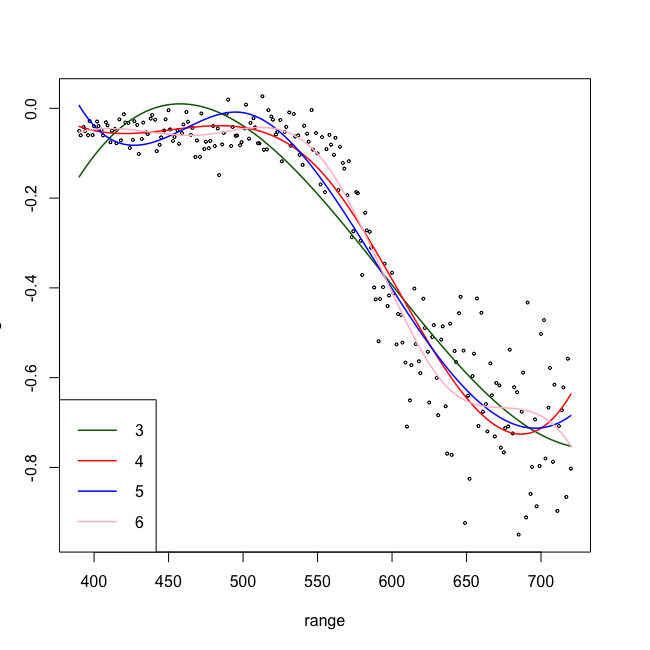
\includegraphics[width = 1\textwidth]{Rplot01.png}
      \end{center}
    \end{figure}
    \textbf{Code:}
    \begin{center}
    \lstinputlisting[basicstyle=\tiny]{r9.txt}
    \end{center} 
    \newpage

    \item[b.] Use a spline with three degrees of freedom to predict the logratio for an observation with range equal to 900,
    Then do the same for a spline with four degrees of freedom. Which prediction do you trust more and why.\\
    \solution Using the predict function in r we can get the prediction for an observation equal to 900. Note that 900
    is outside of the range of data used to build each model. In general this level of extrapolation will likely result in 
    a mediocre prediction, especially with polynomial regressions (and splines). That is why I would expect a more bias model with 
    lower variability to perform better with this prediction i.e. the three degrees of freedom, \\
    \textbf{Code:}
    \begin{center}
    \lstinputlisting[basicstyle=\small]{r5.txt}
    \end{center} 
  \end{enumerate}
 \end{exercise}
 \newpage


\begin{exercise}{3} Use the data frame BigMac2003 in alr4, whcih contains the respoonse Bigmac, of the price of a
  bigmac in various world cities in 2003, expressed in minutes of labor. It also contains quantitative predictors Bread, 
  Rice, Bus, and Apt, which are prices of other goods, as well as economic indicators FoodIndex, TeachGI, TeachNI, TaxRate, 
  and TeachHours.\\
  \begin{enumerate}
    \item[a.] Use principal component analysis on the nine predictors. Report your scree plot and biplot.\\
    \solution Consider the following r code, \\
    \textbf{Code:}
    \begin{center}
    \lstinputlisting[basicstyle=\small]{r6.txt}
    \end{center} 
    \begin{figure}[H]
      \begin{center}
      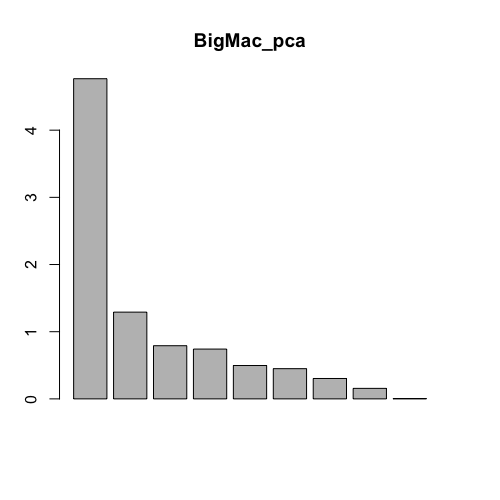
\includegraphics[width = .66\textwidth]{Rplot02.png}
      \end{center}
    \end{figure}
    \begin{figure}[H]
      \begin{center}
      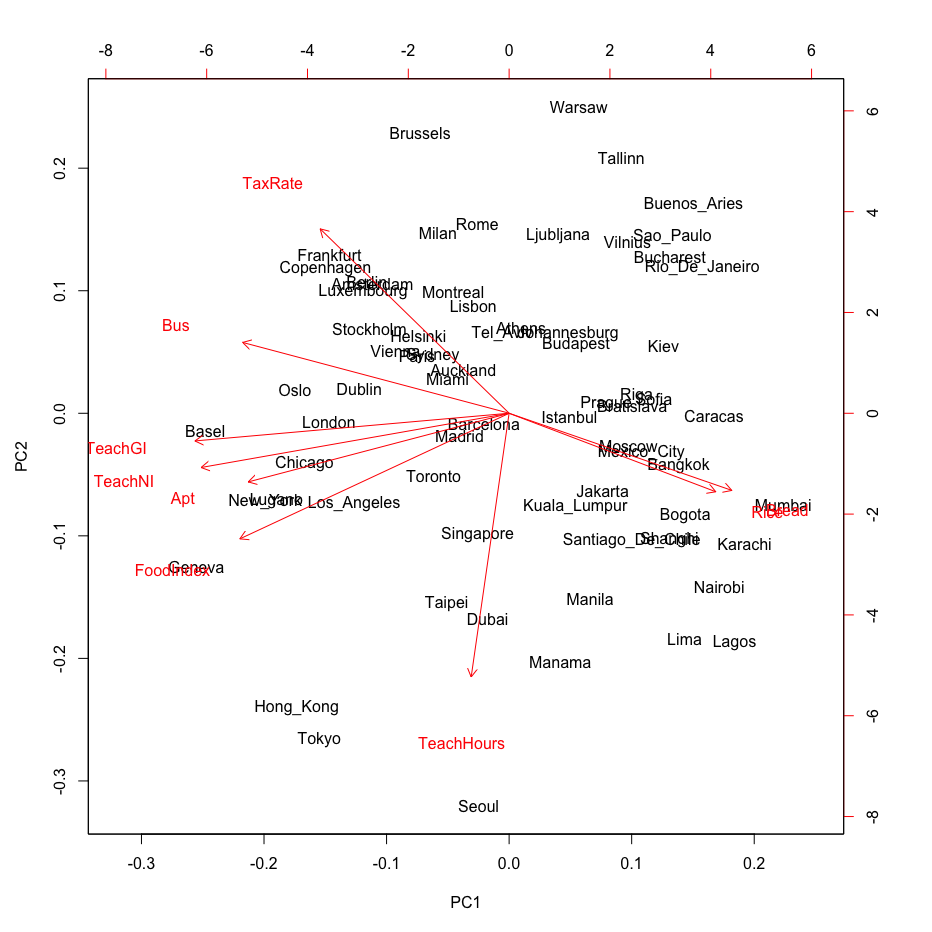
\includegraphics[width = 1\textwidth]{Rplot03.png}
      \end{center}
    \end{figure}
    \newpage

    \item[b.] How many principal components are necessary to use in order to account for at least 90 percent of the variance in 
    the prediction. \\
    \solution Using the summary command in r, we can see the cumulative proportion of variance explained for each PCA,\\
    \textbf{Code:}
    \begin{center}
    \lstinputlisting[basicstyle=\small]{r7.txt}
    \end{center} 
    In order to account for 90 percent of the variance, we should include 6 principle components(we might be able to get away with 5 minding rounding error). 
    \newpage

    \item[c.] Fit the MLR model with the response BigMac and the first four principal components as regressors. Then form the model that 
    contains all nine original predictors. Compare the coefficients of determination for the two models. Are you satisfied that the model with fewer 
    regressors fits sufficiently well compared to the full model?\\
    \solution Fitting the models in r we get, \\
    \textbf{Code:}
    \begin{center}
    \lstinputlisting[basicstyle=\small]{r8.txt}
    \end{center} 
    From the summaries we can see that the PCA model has an coefficient of determination of 0.6137 and the full model including all predictors has 
    a coefficient of determination of 0.6918. Abiding by the principle of parsimony we want to explain the most that we can with the least amount of effort, 
    PCA helps us achieve that, and in that sense this result is very satisfying. 
  \end{enumerate}
  
\end{exercise}



\end{document}





















